\documentclass[12pt,a4paper]{article}

\usepackage[pdftex]{color} 
\usepackage[pdftex]{geometry}
\geometry{hscale=0.78,vscale=0.8}
\usepackage{fancyheadings}
\usepackage{graphicx}
\usepackage{hyperref}
\usepackage{listings}
\usepackage{parskip}

\definecolor{linkColour}{rgb}{0,0.3,0}
\definecolor{urlColour}{rgb}{0,0.3,0}
\definecolor{citeColour}{rgb}{0,0.3,0}

\hypersetup{
  pdftitle={Windmill Hill Observing Guide},
  pdfauthor={Paul Chote, Warwick},
%  pdfpagemode=none,
  pdfborder={0 0 0},
  linkbordercolor={0.5 0.57 0.72},
  colorlinks=true,
  linkcolor=linkColour,
  urlcolor=urlColour,
  citecolor=citeColour
}

%% Definitions

\definecolor{highlightColour}{rgb}{0.7,0,0}

\newcommand{\high}[1]{\textcolor{highlightColour}{#1}}


\pagestyle{fancy}
\begin{document}

\section{Introduction}

The telescope and observatory consist of several sub-systems that work together to deliver images of the sky. They are displayed graphically in Figure \ref{fig:subsystems}, and described in detail below.

\begin{figure}
    \centering
    %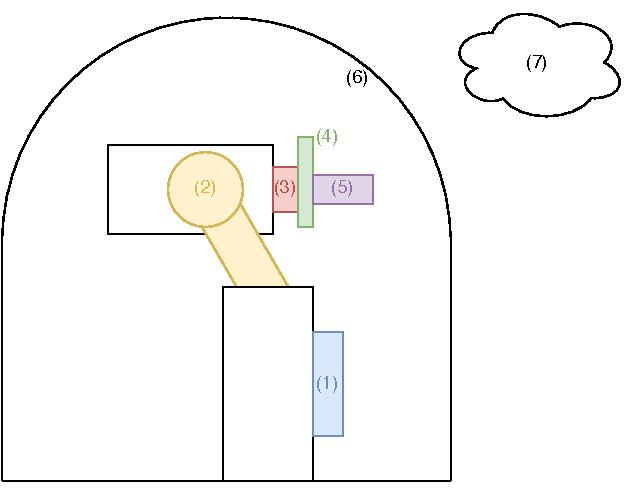
\includegraphics[width=5cm]{figures/subsystems.svg}
    \caption{Schematic overview of the Windmill Hill Observatory systems. (1) power control, (2) telescope mount, (3) focuser, (4) filter wheel, (5) camera, (6) dome, (7) environment monitoring}
    \label{fig:subsystems}
\end{figure}

\subsection{Power Control}

The equipment cabinet mounted on the back of the pier contains (among other things) a network-controllable power board. This is used to remotely power on and off the telescope and instrument components through computer control. This is done using the \texttt{power} command, which will be explained in Section \ref{sec:startup}.

\subsection{Telescope Mount}

The telescope mount is the fork structure that holds the Optical Tube Assembly (OTA) - the actual telescope part of the telescope - and provides computer control to point the telescope at the desired target and to automatically track the sidereal motion of the stars. It can be controlled using the \texttt{tel} command.

\subsection{Focuser}

The focuser is mounted on the back of the OTA, and provides very fine computer control to move the camera in and out to precisely align the camera detector with the image plane of the telescope optics. This alignment changes due to the thermal expansion and contraction of the metal telescope tube, which changes the separation of the primary and secondary mirrors when the temperature changes.

This effect is small in absolute terms (fractions of a millimetre), but has a large impact on the focus of the camera.

\subsection{Filter Wheel}

Most astronomical cameras are monochrome (``black and white'') because they are generally more sensitive and higher resolution than equivalent colour cameras.

Colour images are instead created by placing a piece of coloured glass (called a ``filter'') in front of the camera sensor. Single images can be taken each with a different filters, and combined into a single colour image using software.

The \emph{filter wheel} device sits between the focuser and camera, and contains several different filters that can be selected under computer control.

\subsection{Camera}

The core component of a camera is the sensor that captures light and converts millions of individual brightness measurements into a two-dimensional image.

Traditionally, astronomical cameras generally used sensors based on the Charge Coupled Device (CCD) technology. Until recently, these offered much higher sensitivity and stability than the CMOS sensors used in consumer electronics, but were significantly (factors of $10^3 - 10^6$) more expensive.

By $\sim$2015, advancements in the CMOS technology meant that they were becoming more and more suitable for astronomical use, and had several advantages that made them \emph{more} desirable than CCDs for particular types of observation.

The camera at Windmill Hill contains a 60MP CMOS sensor that is cooled to 0$\circ$C to reduce the impact of thermal noise (called \emph{dark current}) on the images. It contains a very accurate clock, synchronised with the GPS satellite network, to measure the starting and ending times of each image to an accuracy of $\sim$1 millisecond.

\subsection{Dome}

The dome protects the telescope from the sun and weather during the day, and shelters it from the wind (which can cause image shaking) when observing. It contains a shutter that can be opened through computer control, and automatically rotates to allow the telescope to observe through the opening.

It takes 2-3 minutes for the shutter to fully open or close, so be mindful of the weather before you consider opening. If it starts raining, things will get wet before it closes!

\subsection{Environment Monitoring}

A weather mast on the terrace contains a collection of sensors to measure the temperature, humidity, wind speed, cloud coverage, and whether or not it is raining. These measurements allow the dome, when operated robotically (see Section \ref{sec:roboticobserving}), to automatically close when conditions become unsafe.

\section{Operating the telescope}

The Windmill Hill telescope is 100\% computer controlled - there is no eye piece, nor is it necessary to manually rotate or open the dome.

The system is operated using a web browser, with the web dashboard (see Figure \ref{fig:dashboard}) providing an overview of the current status of all systems, and a remote desktop window into the telescope control computer (TCS).

\begin{figure}
    \centering
    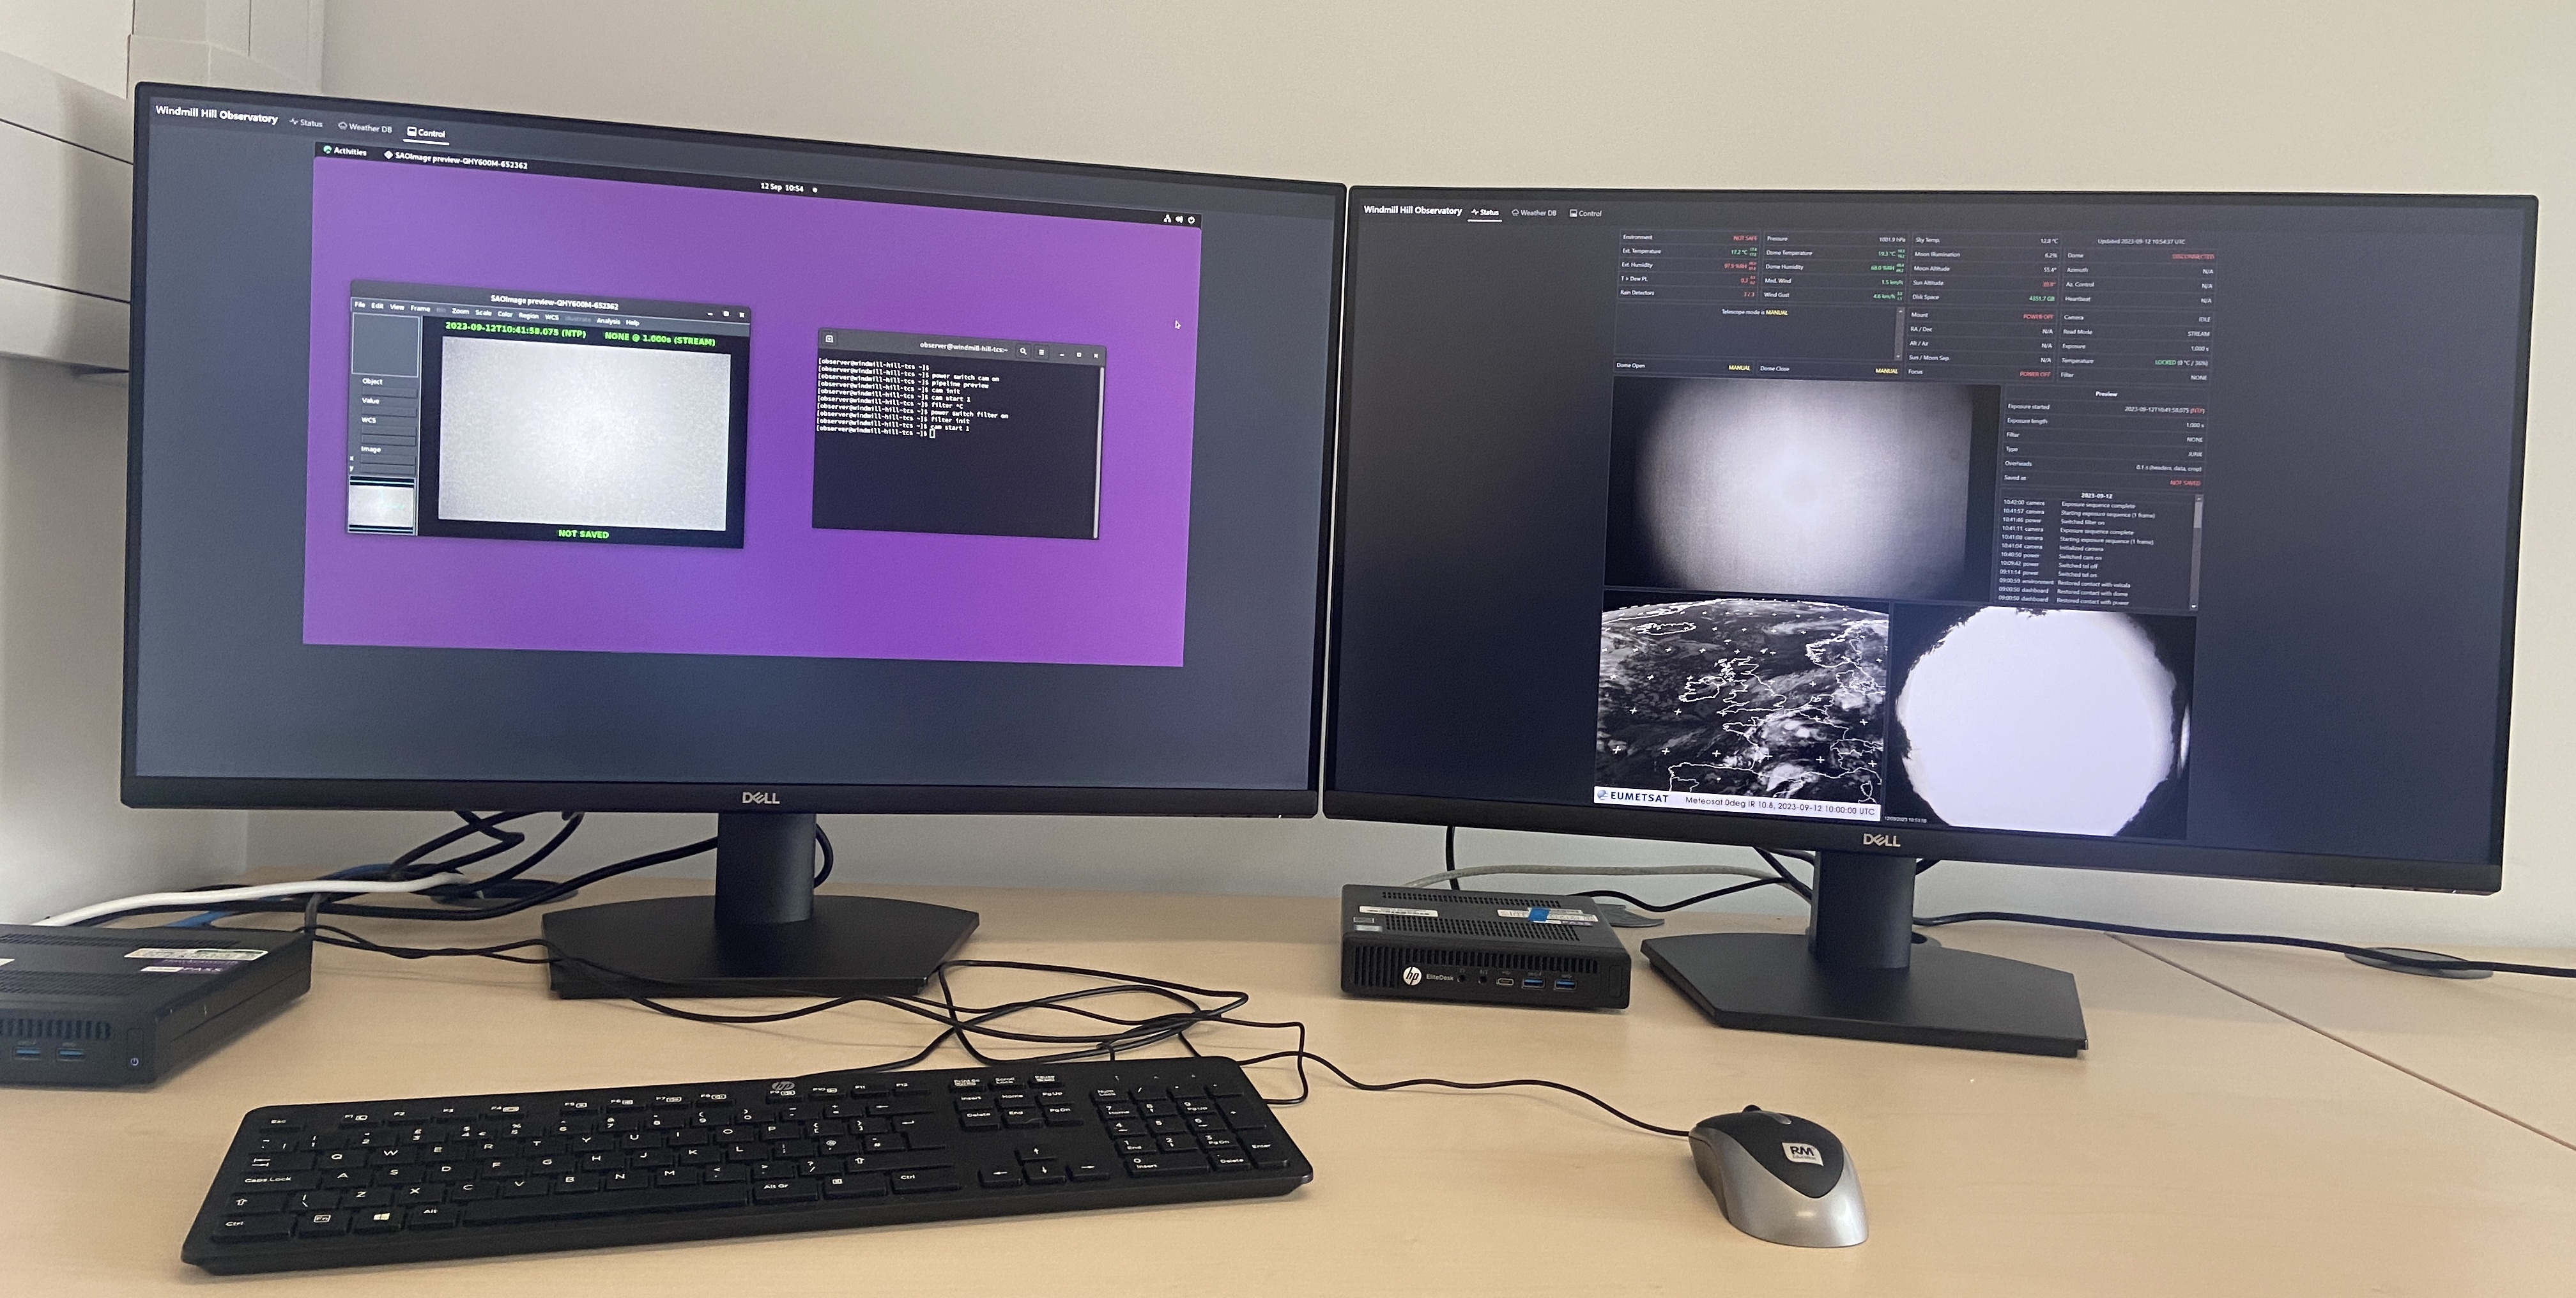
\includegraphics[width=16cm]{figures/dashboard.jpg}
    \caption{The web dashboard interface allows a user to monitor the observatory status and command the telescope.}
    \label{fig:dashboard}
\end{figure}

Log into the control room computer using your ITS account, and open a \emph{Google Chrome} web browser window. Enter the address \texttt{http://172.19.0.160/} to access the dashboard.

It is recommended to use two full screen windows, with one monitor displaying the \emph{Status} page and the other the \emph{Control} page.

The Control page will ask for a password to connect to the TCS; enter \textbf{obs@who} to continue. If presented with a login interface, select the \textbf{observer} user and enter the same password again.

The TCS runs the Rocky Linux operating system, with the Gnome desktop environment. Commands to operate the observatory are entered in a terminal window; if a terminal is not already present on the desktop, press the \textbf{Activities} button at the top-left of the screen, and then the \textbf{Terminal} icon in the dock at the bottom of the Activities overview.

\subsection{Starting Up}\label{sec:startup}

The dome must be powered on and off manually, using a switch on the wall of the telescope room (see Figure \ref{fig:domepower}. Turn it anti-clockwise to the horizontal position to enable power, and clockwise to the vertical position to disable power.

\begin{figure}
    \centering
    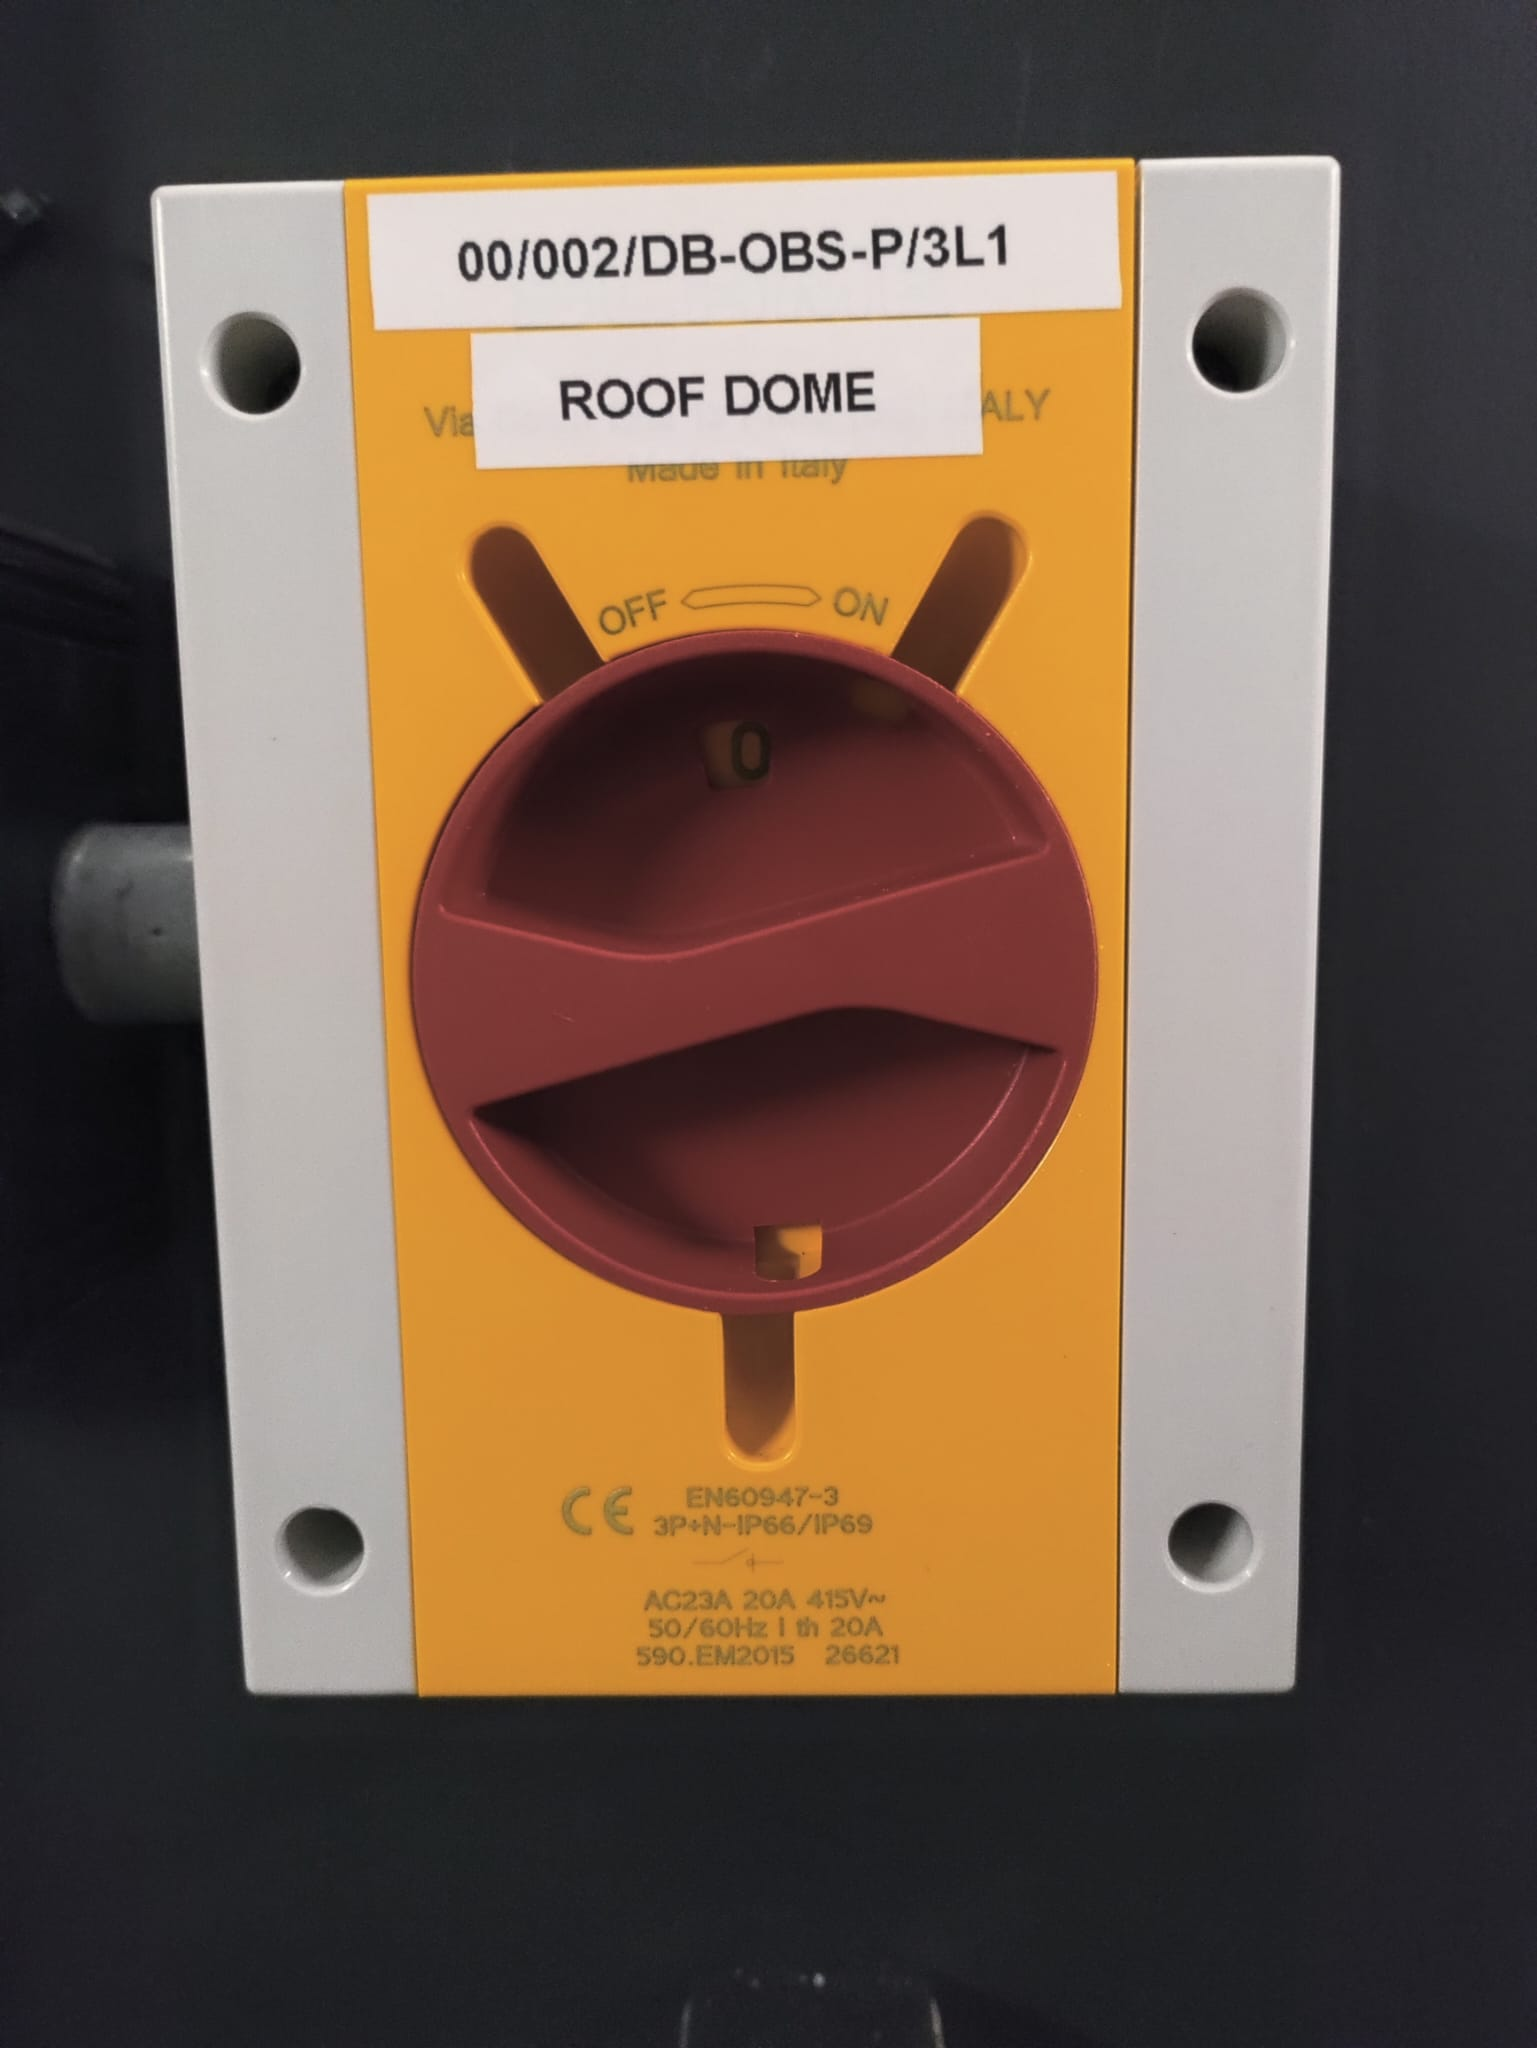
\includegraphics[width=5cm]{figures/domepower.jpg}
    \caption{The switch in the telescope room to turn on the Dome.}
    \label{fig:domepower}
\end{figure}

\subsection{Manual Observing}

\subsection{Robotic Observing}\label{sec:roboticobserving}
\end{document}